\documentclass[journal]{IEEEtran}

\usepackage[utf8]{inputenc}
\usepackage[T1]{fontenc}
\usepackage{amsmath, amsfonts, amssymb}
\usepackage{booktabs}
\usepackage{cite}
\usepackage{graphicx}
\usepackage{bm}
\usepackage{hyperref}
\usepackage{array}
\usepackage{multirow}
\usepackage{placeins}
\usepackage{tabularx}
\usepackage{stfloats}
\usepackage[english]{babel}
\usepackage{microtype}
\emergencystretch=2em

\makeatletter
\renewcommand{\thetable}{\arabic{table}}
\renewcommand{\fnum@table}{Table \thetable.}
\long\def\@makecaption#1#2{%
\ifx\@captype\@IEEEtablestring%
\footnotesize\bgroup%
\setbox\@tempboxa\hbox{\normalfont\footnotesize {#1}\nobreakspace #2}%
\ifdim \wd\@tempboxa >\hsize%
\setbox\@tempboxa\hbox{\normalfont\footnotesize {#1}\nobreakspace}%
\parbox[t]{\hsize}{\normalfont\footnotesize\noindent\unhbox\@tempboxa#2}%
\else%
\hbox to\hsize{\normalfont\footnotesize\box\@tempboxa\hfil}%
\fi%
\par\addvspace{0.5\baselineskip}\egroup%
\@IEEEtablecaptionsepspace%
\else%
\@IEEEfigurecaptionsepspace%
\setbox\@tempboxa\hbox{\normalfont\footnotesize {#1.}\nobreakspace\nobreakspace #2}%
\ifdim \wd\@tempboxa >\hsize%
\setbox\@tempboxa\hbox{\normalfont\footnotesize {#1.}\nobreakspace\nobreakspace}%
\parbox[t]{\hsize}{\normalfont\footnotesize\noindent\unhbox\@tempboxa#2}%
\else%
\hbox to\hsize{\normalfont\footnotesize\box\@tempboxa\hfil}%
\fi%
\fi}
\makeatother

\begin{document}
\raggedbottom

\title{STANet: Sample-Wise Modality Gating for Spatio-Temporal Traffic Anomaly Detection in Intelligent Transport Systems}

\author{
    Ayhan~Gültekin$^{1}$ $|$ Kerem~Kartal$^{2}$ $|$ Ahmet~Yusuf~Şimşek$^{3}$ $|$ Rümeysa~Yeşilova$^{3}$ $|$ Ahmet~Sayar$^{4}$ \\[2ex]
    \small
    $^{1}$Student Affairs Department, Kocaeli University, Kocaeli, Türkiye $|$
    $^{2}$Department of Software Engineering, Kocaeli University, Kocaeli, Türkiye $|$
    $^{3}$Department of Artificial Intelligence and Machine Learning, Kocaeli University, Kocaeli, Türkiye $|$
    $^{4}$Department of Artificial Intelligence Engineering, Bahçeşehir University, Istanbul, Türkiye \\[1.5ex]
    \textbf{Correspondence:} Ayhan Gültekin (ayhan.gultekin@kocaeli.edu.tr)
}

\maketitle

\begin{abstract}
  Traffic anomaly detection is a critical requirement for safe and efficient Intelligent Transportation Systems (ITS), particularly for real-time monitoring and incident response. However, many existing approaches exhibit contextual blindness because they rely on either isolated kinematic signals or static graph representations. This paper presents the \textbf{Spatio-Temporal Adaptive Network (STANet)}, a modality-gated spatio-temporal framework that jointly learns vehicle dynamics and road-topology context for traffic anomaly detection. The architecture combines a stacked Long Short-Term Memory (LSTM) branch with a Graph Attention Network (GAT) branch through a \textbf{sample-wise scalar modality gate} between projected temporal and spatial representations. The gate produces one scalar per sample and applies it uniformly across the complete 64-dimensional embeddings. Experiments on a \textbf{physics-informed synthetic vehicle trajectory dataset} over one \textbf{OpenStreetMap (OSM)}-derived urban network show that STANet achieves \textbf{0.9814 ROC-AUC} and \textbf{0.8282 F1-score}, outperforming the evaluated single-modality baselines and a preliminary diffusion-convolution spatial-encoder variant. A sanity check against a zero-parameter threshold-rule classifier indicates that the model's predictions are not reducible solely to the explicit generation thresholds. These simulation-based findings suggest that STANet may provide a basis for future traffic-monitoring applications following validation on real-world sensor data, external cities, and prospective traffic streams.
\end{abstract}

\begin{IEEEkeywords}
  Traffic Anomaly Detection, Spatio-Temporal Modeling, Graph Attention Network (GAT), Long Short-Term Memory (LSTM), Attention-Gated Fusion, Intelligent Transportation Systems.
\end{IEEEkeywords}

\section{Introduction}

Intelligent Transportation Systems (ITS) have become a fundamental component of modern urban mobility management by enabling large-scale monitoring and analysis of traffic conditions through heterogeneous data sources. These systems generate massive volumes of spatio-temporal traffic data, providing new opportunities for understanding driving behavior and enhancing road safety. Traffic anomalies—such as sudden stops or abnormal maneuvers—can disrupt traffic flow and create significant safety risks. Accurate and timely detection is therefore critical for decision-support mechanisms in ITS environments.

Recent studies have leveraged deep learning, particularly \textbf{Long Short-Term Memory (LSTM)} networks, to model sequential vehicle trajectories. However, road segments form complex graph-structured networks, making purely temporal reasoning insufficient for context-sensitive anomaly detection. To capture structural dependencies, \textbf{Graph Attention Networks (GAT)} and related graph-based approaches have been increasingly adopted alongside temporal encoders. As reflected in recent literature, current research increasingly moves toward both richer spatio-temporal anomaly modeling and more effective fusion strategies for integrating temporal behavior with spatial context \cite{huang_multivariate_2024, sun_framework_2025, nguyen_spatiotemporal_2026, liang_anomaly_2025}. Despite this progress, reliable detection remains challenging because contextual and environmental factors are often underrepresented. Existing approaches frequently suffer from \textbf{``contextual blindness,''} where a model flags natural behavior as anomalous due to limited structural awareness, while many multimodal methods still rely on static or weakly adaptive fusion that cannot fully respond to changing traffic conditions \cite{sun_framework_2025, liang_anomaly_2025}.

To address these limitations, this study introduces the \textbf{Spatio-Temporal Adaptive Network (STANet)}, which integrates a stacked LSTM with a GAT and directly targets the main gaps identified above. The proposed framework jointly models behavioral evolution and road-topology context within a unified spatio-temporal architecture, while replacing static branch combination with a \textbf{sample-wise scalar modality gate} that adaptively balances the complete temporal and spatial embeddings at decision time. Therefore, the main contribution is not merely the coexistence of LSTM and GAT branches, but an explicit decision-level mechanism that determines which modality should dominate for each sample. The main contributions are:
\begin{itemize}
  \item \textbf{Gap-Driven Hybrid Design:} A unified spatio-temporal framework that addresses the limitations of temporal-only, spatial-only, and statically fused hybrid models within a single anomaly-detection pipeline.
  \item \textbf{Sample-Wise Scalar Modality Gating:} A decision-level mechanism that generates one scalar per sample to modulate the complete projected temporal and spatial embeddings instead of using feature-wise, time-step-wise, graph-neighborhood, or fixed fusion weights.
  \item \textbf{Context-Aware Yet Transferable Feature Integration:} Explicit use of OpenStreetMap (OSM) topology together with generic vehicular signals, enabling the model to leverage road context without depending on dataset-specific handcrafted attributes.
  \item \textbf{Interpretable Decision Support:} Gate weights and feature-sensitivity analysis that provide evidence about whether an anomaly is primarily driven by temporal irregularities or local spatial context.
\end{itemize}

\section{Related Work}
The literature most relevant to this study covers both anomaly-detection models and the fusion strategies used to integrate temporal and spatial information. Together, these studies clarify the main gap addressed by STANet: the field increasingly recognizes the need for joint temporal--spatial reasoning, yet many methods still lack an explicitly adaptive mechanism for balancing these two information sources at decision time.

\subsection{Temporal, Spatial, and Spatio-Temporal Anomaly Models}
Early traffic anomaly detection studies were predominantly driven by temporal modeling, where recurrent architectures such as LSTM-based networks were used to capture abrupt variations in velocity, acceleration, and short-term driving behavior. These models remain effective when anomalies are primarily reflected in kinematic changes, but they often overlook whether a maneuver is contextually plausible for the surrounding road environment. In parallel, graph-based and spatially aware methods improved structural understanding by modeling road connectivity, segment interactions, and topological constraints. Such approaches are better suited to representing where risky conditions may emerge, yet they can miss the sequential behavioral evolution that distinguishes a routine slowdown from a truly hazardous event.

Recent studies increasingly bridge these two views through spatio-temporal learning. Huang et al. \cite{huang_multivariate_2024} combine Dynamic GAT and Informer components to capture long-range temporal dependencies together with adaptive relational structure, demonstrating the benefit of graph-temporal interaction for anomaly-sensitive modeling. Duan et al. \cite{sun_framework_2025} extend this direction through a multimodal deep-fusion framework with heterogeneous graph neural networks, enabling joint reasoning over traffic flow, speed, and contextual signals. Nguyen et al. \cite{nguyen_spatiotemporal_2026} further show that graph-based spatio-temporal integration can effectively represent coupled speed--volume patterns in urban traffic environments. Taken together, these studies confirm that anomaly detection benefits from combining behavioral evolution with structural context; however, they still leave open the question of how much weight each modality should receive under changing traffic conditions.

\subsection{Fusion Strategies and Context Integration}
Beyond simply combining temporal and spatial encoders, a second research direction focuses on how information from these branches should be fused and how contextual road knowledge should be injected into the decision process. In this line of work, the central challenge is no longer whether multimodal learning is useful, but whether the fusion mechanism can respond flexibly to scenario-dependent evidence. Liang et al. \cite{liang_anomaly_2025} adopt a lightweight spatio-temporal architecture that emphasizes compact feature fusion, whereas Cui et al. \cite{cui_lane-flow-learning_2026} use a spatial--temporal attention design for lane-aware trajectory prediction. These studies show that attention and feature-level coupling improve representation quality, yet the relative contribution of temporal and spatial cues is still largely determined by architectural configuration rather than by an explicit adaptive gate at inference time.

STANet is positioned within this second strand through a \textbf{sample-wise scalar modality gate} between independently encoded temporal and spatial representations. Huang et al. \cite{huang_multivariate_2024} employ gated attention within an integrated Dynamic GAT--Informer graph-temporal architecture, whereas STANet applies its gate only after the LSTM and GAT outputs have been projected into a shared 64-dimensional space. The proposed $g_{gate}$ is therefore a modality-level selector: it produces one scalar for each sample and broadcasts that value across all latent features. It is not a feature-level attention vector, a time-step attention mechanism, or a graph-neighborhood coefficient. Table \ref{tab:comparison} summarizes this distinction.

\begin{table*}[!t]
\centering
\caption{Summary of related spatio-temporal anomaly detection methods}
\label{tab:comparison}
\renewcommand{\arraystretch}{1.25}
\footnotesize
\setlength{\tabcolsep}{3pt}
\begin{tabularx}{0.97\textwidth}{@{}>{\raggedright\arraybackslash}p{0.15\textwidth}>{\centering\arraybackslash}p{0.06\textwidth}>{\raggedright\arraybackslash}X>{\raggedright\arraybackslash}X>{\raggedright\arraybackslash}X>{\raggedright\arraybackslash}X@{}}
  \toprule
  \textbf{Study} & \textbf{Year} & \textbf{Core Arch.} & \textbf{Temporal} & \textbf{Spatial} & \textbf{Fusion} \\ \midrule
  Huang et al.~\cite{huang_multivariate_2024} & 2024 & Dynamic GAT--Informer & Informer & Dynamic GAT & Integrated gated feature fusion with graph-neighborhood attention \\
  Duan et al.~\cite{sun_framework_2025} & 2025 & Multimodal deep fusion + HGNN & Traffic flow / speed dynamics & Heterogeneous GNN & Integrated multimodal feature fusion \\
  Nguyen et al.~\cite{nguyen_spatiotemporal_2026} & 2026 & Spatiotemporal prediction model & Time-series analysis & Graph-based dependency modeling & Integrated spatio-temporal feature fusion \\
  Liang et al.~\cite{liang_anomaly_2025} & 2025 & Lightweight ST network & TCN / CNN & Spatio-temporal features & Compact feature-level fusion \\
  Cui et al.~\cite{cui_lane-flow-learning_2026} & 2026 & Lane-flow fusion attention & Temporal self-attention & Lane-level spatial attention & Feature-level attention fusion \\
  
  \textbf{STANet (Proposed)} & \textbf{2026} & \textbf{Hybrid LSTM--GAT architecture} & \textbf{Stacked LSTM} & \textbf{Adaptive topology GAT} & \textbf{Modality-level gated fusion: one scalar per sample} \\ \bottomrule
\end{tabularx}
\end{table*}

The fusion labels in Table~\ref{tab:comparison} identify the level at which weighting or interaction occurs. Static concatenation or summation uses no data-dependent weight; integrated feature fusion combines internal representations within a joint architecture; feature-level attention learns dimension- or token-specific weights; graph-neighborhood attention weights adjacent nodes; and modality-level gated fusion controls the relative contribution of complete branch embeddings. STANet belongs to the final category and should not be distinguished merely by the word ``dynamic.''

\FloatBarrier

\section{Problem Formulation}

Urban traffic systems can be modeled as complex spatio-temporal processes in which vehicle movements evolve while simultaneously occurring within the structural constraints of a road network \cite{zhang_automatic_2022, zhang_traffic_2025}. In this study, the traffic anomaly detection problem is formulated as a context-aware learning task that jointly models vehicle trajectory dynamics and road network topology, addressing the challenges of high-dimensional coupling and temporal dynamics inherent in such systems \cite{ren_graph_2024}. The mathematical notations used throughout this formulation are summarized in Table \ref{tab:notations}.

\begin{table}[!htbp]
  \centering
  \caption{Summary of mathematical notation}
  \label{tab:notations}
  \renewcommand{\arraystretch}{1.2}
  \begin{tabular}{@{}p{0.36\columnwidth}p{0.58\columnwidth}@{}}
    \toprule
    \textbf{Symbol} & \textbf{Description} \\ \midrule
    $\mathcal{G} = (\mathcal{V}, \mathcal{E})$ & Directed graph representing the road network \\
    $\mathcal{V}, \mathcal{E}$ & Set of nodes (road segments) and edges (connectivity) \\
    $N, \mathbf{A}$ & Number of nodes and adjacency matrix encoding connectivity \\
    $\mathbf{s}_i, \mathcal{S}$ & Structural feature vector of node $i$ and the set of all structural features \\
    $\mathcal{T} = \{\mathbf{x}_1, \dots, \mathbf{x}_\tau\}$ & Vehicle trajectory sequence of length $\tau$ \\
    $\mathbf{x}_t, \mathbf{X} \in \mathbb{R}^{\tau \times 4}$ & Per-step kinematic vector and stacked temporal feature matrix \\
    $v_t, a_t, \theta_t, id_t$ & Velocity, acceleration, heading angle, and road-segment ID at time $t$ \\
    $x_{sin}, x_{cos}$ & Trigonometric heading components used for continuous angular representation \\
    \shortstack[l]{$type_i, length_i$\\$deg_i, context_i$} & \shortstack[l]{Road category and segment length;\\node degree and contextual attributes} \\
    $\mathbf{h}_t, \mathbf{h}_{temp}, \mathbf{h}_{spat}$ & LSTM hidden state, temporal embedding, and spatial embedding \\
    $\Theta_{temp}, \Theta_{spat}$ & Learnable parameter sets of the LSTM and GAT branches \\
    $\alpha_{ij}, \mathcal{N}_i$ & Graph-attention coefficient from node $j$ to node $i$ and neighborhood of node $i$ \\
    $\mathbf{W}, \vec{a}, \mathbf{h}_i'$ & GAT transform matrix, attention vector, and updated node representation \\
    $d$ & Shared latent dimension used before multimodal fusion \\
    $\mathbf{h}'_{temp}, \mathbf{h}'_{spat}$ & Projected temporal and spatial embeddings in shared latent space \\
    \shortstack[l]{$\mathbf{W}_t, \mathbf{b}_t$\\$\mathbf{W}_s, \mathbf{b}_s$} & Learnable projection parameters for temporal/spatial branches \\
    $g_{gate}, \mathbf{W}_g, b_g$ & Sample-wise scalar modality weight and gating-network parameters \\
    $\mathbf{z}$ & Joint spatio-temporal fused embedding \\
    \shortstack[l]{$f_{LSTM}(\cdot), f_{GAT}(\cdot)$\\$f_{fusion}(\cdot), g(\cdot)$} & \shortstack[l]{Temporal encoder, spatial encoder,\\fusion, and classification mappings} \\
    $\sigma(\cdot)$ & Activation function (sigmoid where specified) \\
    \shortstack[l]{$y, \hat{y}$\\$y_i, \hat{y}_i$} & Ground-truth and predicted labels (global and sample-level forms) \\
    $\mathcal{L}, M$ & Loss function and mini-batch size \\
    $w_{pos}$ & Positive-class weight in the WBCE loss \\
    $\Phi$ & Overall mapping function for anomaly detection \\ \bottomrule
  \end{tabular}
\end{table}

\subsection{Road Network Representation}
The road network is represented as a directed graph $\mathcal{G} = (\mathcal{V}, \mathcal{E})$, where $\mathcal{V}$ is a set of $N$ nodes (road segments) and $\mathcal{E}$ denotes the set of edges representing physical connectivity \cite{li_graph_2023, park_graph_2025}. Each node $v_i \in \mathcal{V}$ is associated with a structural feature vector $\mathbf{s}_i$ that captures the contextual properties of the segment:
\begin{equation}
  \mathbf{s}_i = [type_i, length_i, deg_i, context_i]
\end{equation}
where $type_i$ denotes the road category, $length_i$ is the segment length, $deg_i$ is the node degree (connectivity count), and $context_i$ represents additional intersection characteristics \cite{chen_enhancing_2026, zhong_multi-factor_2025}. Spatial dependencies are encoded via an adjacency matrix $\mathbf{A}$, which can be extended to an adaptive structure to capture time-varying spatial correlations \cite{pan_dc-stgcn_2021, chang_stfdsgcn_2025}.

\subsection{Vehicle Trajectory Modeling}
Vehicle movement is represented as a trajectory sequence $\mathcal{T} = \{\mathbf{x}_1, \mathbf{x}_2, \dots, \mathbf{x}_\tau\}$, where $\tau$ is the sequence length and each observation $\mathbf{x}_t$ describes the kinematic state at time $t$ \cite{zhou_hybrid_2022, taheri_sarteshnizi_applicability_2026}. The feature vector is defined as:
\begin{equation}
  \mathbf{x}_t = [v_t, a_t, \theta_t, id_t]
\end{equation}
where $v_t$ is speed, $a_t$ is acceleration, $\theta_t$ is the heading angle, and $id_t$ is the identifier of the road segment where the vehicle is located. These features capture the temporal evolution of driving behavior.

\subsection{Spatio-Temporal Feature Representation}
Anomaly detection requires the integration of behavioral dynamics and structural context \cite{hu_dynamic_2026, zhu_spatio-temporal_2026}. We define the learning task as finding a joint embedding $\mathbf{z}$ that maps the trajectory and the graph into a latent space:
\begin{equation}
  \mathbf{z} = f(\mathbf{h}_{temp}, \mathbf{h}_{spat})
\end{equation}
where $\mathbf{h}_{temp} = \text{LSTM}(\mathcal{T})$ represents the temporal features and $\mathbf{h}_{spat} = \text{GAT}(\mathcal{G}, \mathbf{A})$ represents the spatial features \cite{xia_attention-based_2023, wang_multi-scale_2025}. The function $f(\cdot)$ denotes a sample-wise scalar modality-gating mechanism that balances the two projected branch representations using one learned scalar per sample \cite{zhao_starg2n_2025}.

\subsection{Traffic Anomaly Detection Objective}
The detection task is formulated as a binary classification. For a given trajectory $\mathcal{T}$ and road context $\mathcal{G}$, the model predicts the probability $\hat{y}$ that the segment is anomalous:
\begin{equation}
  \hat{y} = \sigma(g(\mathbf{z}))
\end{equation}
where $g(\cdot)$ is the classification head and $\hat{y} \in [0, 1]$. At the task-formulation level, binary classification can be expressed using standard unweighted binary cross-entropy:
\begin{equation}
  \label{eq:generic_bce}
  \mathcal{L} = -\frac{1}{M} \sum_{i=1}^{M} [y_i \log(\hat{y}_i) + (1 - y_i) \log(1 - \hat{y}_i)]
\end{equation}
where $y_i \in \{0, 1\}$ is the ground truth label and $M$ is the number of samples \cite{feng_traffic_2024, sun_framework_2025, ma_utfp-ad_2025}.
Equation~\ref{eq:generic_bce} is the generic task-level formulation only. Because the training partition is imbalanced, the implemented optimization objective is the weighted binary cross-entropy in Eq.~\ref{eq:wbce}.

\subsection{Problem Definition}
Given a road network $\mathcal{G}$, vehicle trajectory $\mathcal{T}$, and road features $\mathcal{S}$, the objective is to learn a mapping function $\Phi: \{\mathcal{T}, \mathcal{G}, \mathcal{S}\} \rightarrow \{0, 1\}$ that accurately identifies traffic anomalies by capturing the non-linear spatio-temporal dependencies between driving behavior and road topology \cite{guo_crfpi-net_2026, ren_graph_2024}.

\section{Proposed Method}

This section presents the architecture of the \textbf{Spatio-Temporal Adaptive Network (STANet)}, a context-aware framework designed for traffic anomaly detection. The model jointly learns temporal vehicle dynamics and spatial road network topology to capture high-dimensional dependencies. Its specific fusion contribution is a \textbf{sample-wise scalar modality gate} operating between projected temporal and spatial representations. Unlike feature-level attention, it does not learn a separate coefficient for each of the 64 latent dimensions; unlike temporal attention, it does not assign weights to individual time steps; and unlike GAT neighborhood attention, it does not weight graph neighbors. Instead, it generates one scalar for each sample and uses that value to control the relative contribution of the complete LSTM and GAT embeddings.

As illustrated in Fig. \ref{fig:stanet_framework}, the proposed framework consists of three core components: (i) a Temporal Module for sequence modeling, (ii) a Spatial Module for structural graph learning, and (iii) a Sample-Wise Scalar Modality-Gating Module for context-aware integration.

\subsection{Overall Architecture}
The end-to-end architecture of STANet is illustrated in Fig. \ref{fig:stanet_framework}. The model processes vehicle trajectories and OSM-derived road topology through parallel LSTM and GAT branches, fuses them using a sample-wise scalar modality gate, and maps the resulting representation to anomaly predictions.

\begin{figure*}[t]
  \centering
  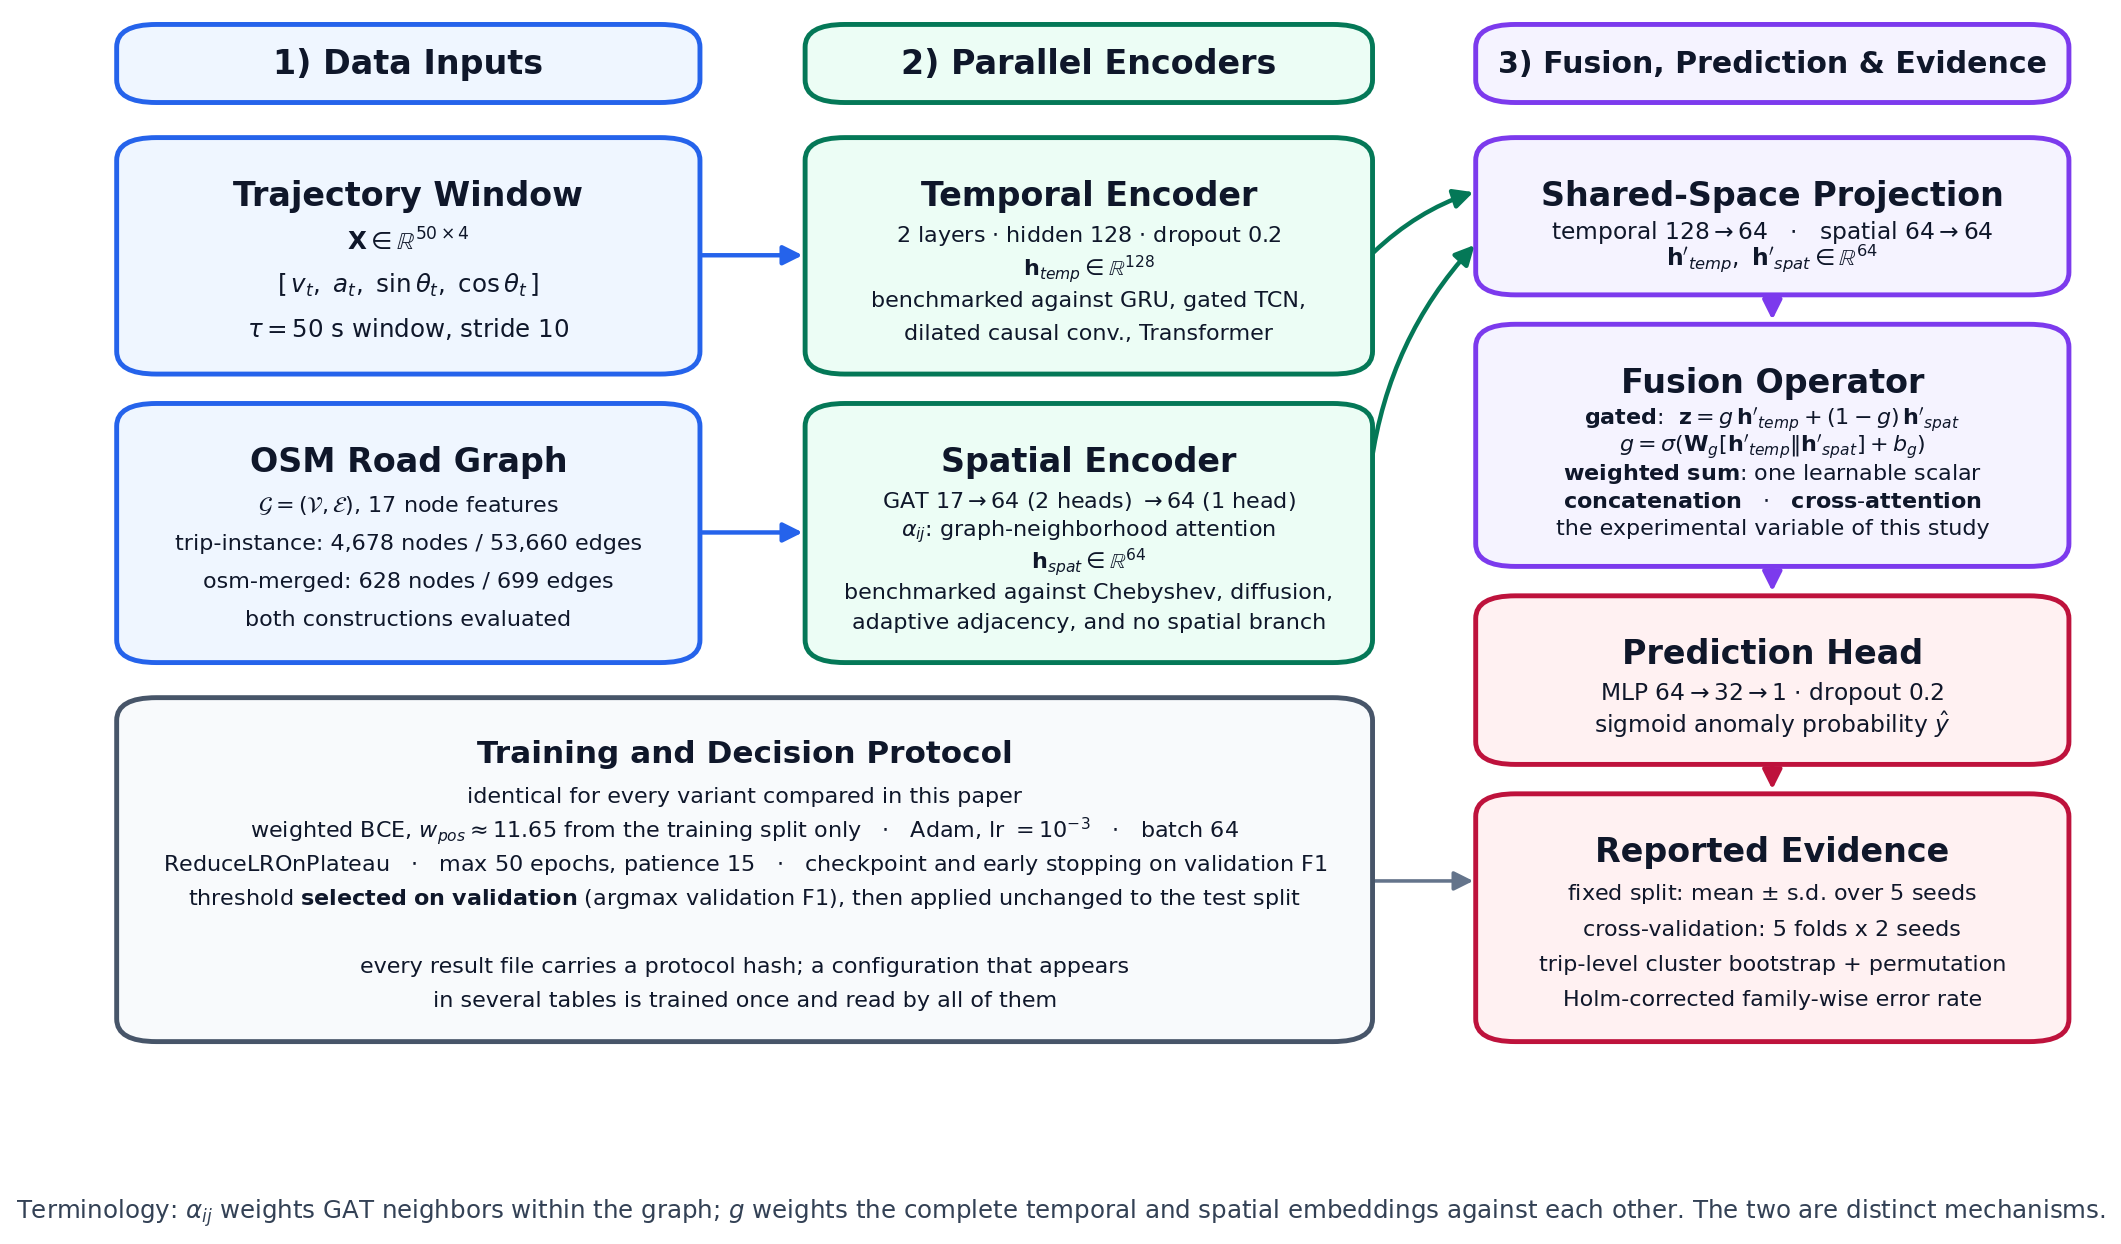
\includegraphics[width=0.98\textwidth]{stanet_framework_q1.png}
  \caption{Overall architecture of STANet. The GAT neighborhood coefficients $\alpha_{ij}$ are distinct from the sample-wise scalar modality gate $g_{gate}$.}
  \label{fig:stanet_framework}
\end{figure*}

Given a vehicle trajectory sequence $\mathcal{T}$ and the road network graph $\mathcal{G}$, the model learns two complementary latent embeddings:
\begin{align}
  \mathbf{h}_{temp} &= f_{LSTM}(\mathcal{T}; \Theta_{temp}) \\
  \mathbf{h}_{spat} &= f_{GAT}(\mathcal{G}, \mathbf{A}; \Theta_{spat})
\end{align}
where $\Theta_{temp}$ and $\Theta_{spat}$ denote the learnable parameter sets of the LSTM and GAT branches, respectively \cite{wang_multi-scale_2025, he_c_2025}. These embeddings are integrated through the scalar modality-gating mechanism:
\begin{equation}
  \mathbf{z} = f_{fusion}(\mathbf{h}_{temp}, \mathbf{h}_{spat})
\end{equation}
The fused representation $\mathbf{z}$ is then utilized by a classification head to predict the final anomaly probability $\hat{y}$.

\subsection{Temporal Module: Trajectory Modeling}

\subsubsection{Kinematic Feature Representation}
The temporal branch processes four fundamental kinematic features to describe vehicle motion at each time step $t$:
\begin{equation}
  \mathbf{x}_t = [v_t, a_t, \sin(\theta_t), \cos(\theta_t)]
\end{equation}
where $v_t$ is velocity and $a_t$ is acceleration. Representing the heading angle $\theta_t$ using its trigonometric components prevents periodic discontinuities at the angular boundaries ($0^\circ$ and $360^\circ$) \cite{taheri_sarteshnizi_applicability_2026}. Accordingly, each driving window is represented as $\mathbf{X} \in \mathbb{R}^{\tau \times 4}$ with $\tau = 50$, enabling the model to capture fine-grained variations in vehicle kinematics over a 50-second observation horizon.

\subsubsection{LSTM-Based Sequence Encoding}
To capture long-term temporal dependencies in driving behavior, STANet employs a two-layer stacked \textbf{Long Short-Term Memory (LSTM)} encoder \cite{zhou_hybrid_2022, taheri_sarteshnizi_applicability_2026, hirata_traffic_2025}. The module is designed to detect microscopic changes in the driving profile by recursively processing the past $\tau$ observations. The hidden state update at time $t$ is defined as:
\begin{equation}
  \mathbf{h}_t = \text{LSTM}(\mathbf{x}_t, \mathbf{h}_{t-1})
\end{equation}
where $\mathbf{x}_t$ denotes the current kinematic vector and $\mathbf{h}_t$ denotes the hidden state summarizing the temporal context observed up to step $t$. Each LSTM layer contains 128 hidden units, and a dropout rate of 0.2 is applied between recurrent layers to mitigate overfitting. In the hybrid setting, the final hidden state of the second layer is exported as the temporal embedding:
\begin{equation}
  \mathbf{h}_{temp} = \mathbf{h}_\tau
\end{equation}
For standalone temporal evaluation, the same 128-dimensional embedding can be passed to a lightweight fully connected layer followed by a sigmoid activation to produce a branch-wise anomaly probability. This design allows the LSTM branch to serve both as a discriminative temporal encoder and as the temporal component used in ablation experiments. Table \ref{tab:lstm_config} summarizes the main settings and tensor transitions of the temporal branch.

\begin{table}[!htbp]
  \centering
  \caption{Summary of LSTM branch configuration}
  \label{tab:lstm_config}
  \renewcommand{\arraystretch}{1.15}
  \resizebox{\columnwidth}{!}{%
  \begin{tabular}{@{}lll@{}}
    \toprule
    \textbf{Component} & \textbf{Setting} & \textbf{Role / Output} \\ \midrule
    Input window & $\tau = 50$, 4 features & Tensor shape $[B, 50, 4]$ \\
    Input features & $v_t$, $a_t$, $x_{sin}$, $x_{cos}$ & Driving-profile representation \\
    Stacked LSTM & input size $=4$, hidden size $=128$ & Temporal dependency learning \\
    Number of layers & 2 & Hierarchical sequence encoding \\
    Dropout & $p = 0.2$ & Regularization between LSTM layers \\
    Temporal embedding & $\mathbf{h}_{temp} \in \mathbb{R}^{128}$ & Output tensor $[B, 128]$ \\
    Branch classifier & Linear $128 \rightarrow 1$ + sigmoid & Branch-wise score $[B, 1]$ \\
    \bottomrule
  \end{tabular}}
\end{table}

\subsection{Spatial Module: Road Topology Learning}

\subsubsection{Graph-Based Contextual Features}
The spatial module utilizes a \textbf{Graph Attention Network (GAT)} to encode the road network structure \cite{zhang_automatic_2022, li_graph_2023, zhong_multi-factor_2025}. The road network is modeled as a directed graph $\mathcal{G} = (\mathcal{V}, \mathcal{E})$, where each node corresponds to a road segment and each edge denotes a feasible physical transition between adjacent segments. Each node $v_i$ is associated with a 17-dimensional structural vector $\mathbf{s}_i$ capturing:
\begin{itemize}
  \item \textbf{Road-type descriptors:} One-hot encoded road categories together with segment-level geometric attributes.
  \item \textbf{Topological metrics:} Betweenness and closeness centrality scores that reflect network importance \cite{zhong_multi-factor_2025}.
  \item \textbf{Contextual constraints:} Traffic-light indicators, tunnel information, and rarity scores that reflect atypical segment usage.
\end{itemize}

\subsubsection{Graph Attention Mechanism}
Unlike standard graph convolutions, the GAT layers compute adaptive attention coefficients $\alpha_{ij}$ to identify the most relevant adjacent road segments \cite{xia_attention-based_2023, ren_graph_2024, chen_gms_2026}:
\begin{equation}
  \alpha_{ij} = \frac{\exp\left(\text{LeakyReLU}\left(\vec{a}^T [\mathbf{W}\mathbf{s}_i \Vert \mathbf{W}\mathbf{s}_j]\right)\right)}{\sum_{k \in \mathcal{N}_i} \exp\left(\text{LeakyReLU}\left(\vec{a}^T [\mathbf{W}\mathbf{s}_i \Vert \mathbf{W}\mathbf{s}_k]\right)\right)}
\end{equation}
where $\Vert$ denotes the concatenation operator. The updated node representation is computed as a weighted sum of neighbor features followed by a non-linear activation $\sigma$:
\begin{equation}
  \mathbf{h}_i' = \sigma \left( \sum_{j \in \mathcal{N}_i} \alpha_{ij} \mathbf{W}\mathbf{s}_j \right)
\end{equation}
STANet employs two consecutive GAT layers with multi-head attention to ensure stable learning of spatial dependencies. The first layer maps the 17-dimensional node attributes to a 64-dimensional intermediate representation using 32 hidden channels and 2 attention heads. The second layer refines this representation and produces the final 64-dimensional spatial embedding. In the hybrid pipeline, the embedding associated with the road segment occupied by the vehicle is extracted as $\mathbf{h}_{spat}$, whereas a lightweight fully connected head can be used for branch-wise spatial anomaly scoring during standalone GNN evaluation. The detailed settings of this spatial branch are summarized in Table \ref{tab:gnn_config}.

\begin{table}[!htbp]
  \centering
  \caption{Summary of GNN branch configuration}
  \label{tab:gnn_config}
  \renewcommand{\arraystretch}{1.15}
  \resizebox{\columnwidth}{!}{%
  \begin{tabular}{@{}lll@{}}
    \toprule
    \textbf{Component} & \textbf{Setting} & \textbf{Role / Output} \\ \midrule
    Graph input & $4{,}678$ nodes, $53{,}660$ edges & Directed OSM-derived road graph \\
    Node features & 17 dimensions & Structural and contextual segment descriptors \\
    GAT layer 1 & GATConv$(17, 32,$ heads$=2)$ & Intermediate tensor $[N, 64]$ \\
    GAT layer 2 & GATConv$(64, 64,$ heads$=1)$ & Spatial embedding tensor $[N, 64]$ \\
    Attention type & Multi-head then single-head & Robust neighborhood weighting \\
    Spatial embedding & $\mathbf{h}_{spat} \in \mathbb{R}^{64}$ & Output of active road segment \\
    Branch classifier & Linear $64 \rightarrow 1$ + sigmoid & Branch-wise score $[N, 1]$ \\
    \bottomrule
  \end{tabular}}
\end{table}

\subsection{Sample-Wise Scalar Modality-Gating Module}
The specific fusion contribution of STANet is a \textbf{sample-wise scalar modality gate} that integrates temporal and spatial features in a shared latent space \cite{zhao_starg2n_2025, pan_dc-stgcn_2021}.

\subsubsection{Projection into Shared Space}
Since $\mathbf{h}_{temp}$ and $\mathbf{h}_{spat}$ originate from different architectural branches, they are first projected into a common latent dimensionality $d = 64$:
\begin{align}
  \mathbf{h}'_{temp} &= \text{ReLU}(\mathbf{W}_t \mathbf{h}_{temp} + \mathbf{b}_t) \\
  \mathbf{h}'_{spat} &= \text{ReLU}(\mathbf{W}_s \mathbf{h}_{spat} + \mathbf{b}_s)
\end{align}
where $\mathbf{W}_t \in \mathbb{R}^{64 \times 128}$ aligns the temporal embedding with the shared fusion space and $\mathbf{W}_s \in \mathbb{R}^{64 \times 64}$ preserves the spatial embedding in the same space. This projection stage ensures dimensional compatibility before adaptive weighting.

\subsubsection{Scalar Modality-Gate Calculation}
A gating network computes $g_{gate}$, which determines the relative importance of the projected temporal and spatial modalities \cite{zhang_context-aware_2025}. To avoid confusion with the graph-neighborhood attention coefficients $\alpha_{ij}$ used inside the GAT layers, the modality-gate output is explicitly denoted by $g_{gate}$:
\begin{equation}
  g_{gate} = \sigma(\mathbf{W}_g [\mathbf{h}'_{temp} \Vert \mathbf{h}'_{spat}] + b_g)
\end{equation}
where $g_{gate}\in[0,1]$ has tensor shape $[B,1]$ for a batch of size $B$. Thus, exactly one scalar is generated for each sample and broadcast across all 64 dimensions of both projected embeddings. A value closer to 1 emphasizes the complete temporal representation, whereas a value closer to 0 emphasizes the complete spatial representation. The mechanism is therefore modality-level and sample-wise, rather than feature-level, time-step-level, or graph-neighborhood-level.

\subsubsection{Feature Fusion and Classification}
The final joint spatio-temporal embedding $\mathbf{z}$ is computed via the gated integration:
\begin{equation}
  \mathbf{z} = g_{gate} \cdot \mathbf{h}'_{temp} + (1 - g_{gate}) \cdot \mathbf{h}'_{spat}
\end{equation}
This fused representation is passed through a two-layer Multi-Layer Perceptron (MLP) with ReLU and dropout regularization to generate the anomaly probability:
\begin{equation}
  \hat{y} = \sigma(\text{MLP}(\mathbf{z}))
\end{equation}
The classifier maps the shared 64-dimensional fused vector through a $64 \rightarrow 32 \rightarrow 1$ architecture, with dropout $p = 0.2$ applied before the final sigmoid output. Because the same $g_{gate}$ value multiplies every latent dimension, the gate controls modality contribution but does not perform feature selection within either embedding. The main components of this stage are summarized in Table \ref{tab:fusion_config}.

\begin{table}[!htbp]
  \centering
  \caption{Summary of sample-wise scalar modality-gating configuration}
  \label{tab:fusion_config}
  \renewcommand{\arraystretch}{1.15}
  \resizebox{\columnwidth}{!}{%
  \begin{tabular}{@{}lll@{}}
    \toprule
    \textbf{Component} & \textbf{Setting} & \textbf{Role / Output} \\ \midrule
    Temporal projection & Linear $128 \rightarrow 64$ + ReLU & Shared-space tensor $[B, 64]$ \\
    Spatial projection & Linear $64 \rightarrow 64$ + ReLU & Shared-space tensor $[B, 64]$ \\
    Gate input & Concatenation of projected embeddings & Tensor $[B, 128]$ \\
    Scalar modality gate & Linear $128 \rightarrow 1$ + sigmoid & One weight per sample, shape $[B, 1]$ \\
    Fusion rule & $g_{gate}\mathbf{h}'_{temp} + (1-g_{gate})\mathbf{h}'_{spat}$ & Fused tensor $[B, 64]$ \\
    Classifier & MLP $64 \rightarrow 32 \rightarrow 1$ + ReLU + dropout $0.2$ & Final probability $[B, 1]$ \\
    \bottomrule
  \end{tabular}}
\end{table}

\section{Dataset and Preprocessing}

This section describes the data sources utilized in this study and the preprocessing pipeline developed to ensure data quality. The proposed framework integrates high-fidelity vehicle trajectory data with structural road network information to capture the nuanced spatio-temporal dependencies required for context-aware anomaly detection \cite{zhang_automatic_2022, zhang_traffic_2025}.

\subsection{Data Sources}
The empirical validation of STANet relies on two primary data sources: a \textbf{vehicle trajectory dataset} for behavioral modeling and \textbf{OpenStreetMap (OSM)} for road network topology.

\subsubsection{Vehicle Trajectory Dataset}
\nocite{wen_hdsvt_2025,feng_traffic_2024_dup2,yu_spatio-temporal_2018,li_diffusion_2018,wu_graph_2019,francies_framework_2025,pipes_car_following_1967,aashto_green_book_2018}
To obtain trajectory data with reliable, fully known ground-truth anomaly labels---which are difficult to obtain at scale from real-world sensor logs because of privacy constraints, sparse anomaly incidence, and the absence of verified incident annotations---this study employs a physics-informed synthetic trajectory-generation framework. Vehicle motion is simulated over the OSM-derived Kocaeli road network (Section~\ref{sec:osm_data}) using a Markov-chain-based behavioral model in which each vehicle transitions between four kinematic states (constant speed, acceleration, deceleration, and stop) at one-second resolution. State-transition probabilities are conditioned on the local traffic regime (free-flow, transition, or congested), defined through a log-normal traffic-intensity distribution and an empirically motivated speed--density relationship adapted from Pipes' car-following model \cite{pipes_car_following_1967}:
\begin{equation}
  \bar{v}_s = (v_{\max} - 0.08v_{\max})\left(1-\frac{\tau}{10}\right)^4,
\end{equation}
where $v_{\max}$ is the segment's speed limit and $\tau \in [1,9]$ is the sampled traffic-intensity level. Acceleration values are constrained to a physically realistic envelope of $[-3,1.5]$~m/s$^2$ under normal driving, following AASHTO geometric-design guidance \cite{aashto_green_book_2018}. Sensor-level noise is injected into the speed and bearing channels at every time step to emulate GPS jitter and prevent the model from training on unrealistically clean signals.

This simulation-based design provides controlled ground-truth labels and avoids privacy-sensitive location data. Performance under real sensing noise, traffic behavior, and incident distributions remains to be evaluated using field-collected and cross-city datasets. Sensitivity to the preprocessing and anomaly-generation configuration is considered in Section~\ref{sec:future_directions}.

\subsubsection{OpenStreetMap (OSM) Road Network Data}
\label{sec:osm_data}
To provide the necessary spatial context, the road network is modeled as a graph using data extracted from OpenStreetMap. As defined in the methodology, each road segment is represented by a 17-dimensional feature vector $\mathbf{s}_i$ \cite{zhong_multi-factor_2025}. After preprocessing, the graph used in experiments contains 4,678 nodes and 53,660 directed edges, corresponding to an average node degree of approximately 11.47. These attributes include structural indicators (lane count and road category), infrastructure elements (traffic lights and tunnels), and complex topological measures such as betweenness and closeness centrality \cite{li_graph_2023, zhong_multi-factor_2025}.

Several structural attributes required imputation because of incomplete OSM tagging. Lane counts and speed limits, when missing from OSM, were assigned the road-type-conditional imputation defaults in Table~\ref{tab:road_defaults}; assigned speed values were additionally smoothed using
\begin{equation}
  \begin{aligned}
    \hat{v}_i & =
    \begin{cases}
      \operatorname{Round}_5\!\left(\dfrac{v_{i-1}+v_i+v_{i+1}}{3}\right), & C_i,\\
      v_i, & \text{otherwise},
    \end{cases}\\
    C_i & \equiv (S_i \neq \mathrm{OSM}) \land (|v_{i-1}-v_i|>30),
  \end{aligned}
\end{equation}
to remove physically implausible discontinuities (e.g., abrupt $120\rightarrow70$~km/h transitions) that would otherwise arise from independent per-segment default assignment. Traffic-light presence was inferred using a hybrid rule combining direct OSM \texttt{traffic\_signals} tags with a node-degree heuristic: intersections with degree $\geq4$, excluding motorway and link segments, are treated as signal-controlled.

The values in Table~\ref{tab:road_defaults} are \textbf{author-defined simulation and imputation assumptions}. They are not observed OSM attributes, are not presented as Turkish statutory limits, and were not derived from a formal calibration study. Their purpose is to provide deterministic fallback values when tags are absent. The present experiments do not include a sensitivity analysis for these defaults; consequently, dependence on the assumed lane counts and speed limits remains an open methodological limitation.

\begin{table}[!htbp]
  \centering
  \caption{Author-defined road-type-conditional imputation defaults}
  \label{tab:road_defaults}
  \renewcommand{\arraystretch}{1.15}
  \begin{tabular}{@{}lcc@{}}
    \toprule
    \textbf{Road Type} & \textbf{Default Lanes} & \textbf{Default Speed (km/h)} \\ \midrule
    motorway        & 3  & 130 \\
    motorway\_link  & 1  & 80 \\
    trunk           & 2  & 110 \\
    trunk\_link     & 1  & 60 \\
    primary         & 2  & 90 \\
    primary\_link   & 1  & 50 \\
    secondary       & 1  & 80 \\
    secondary\_link & 1  & 40 \\
    (default)       & -- & 50 \\ \bottomrule
  \end{tabular}
\end{table}

The resulting network covers 10 central districts of Kocaeli, Türkiye (İzmit, Gebze, Körfez, Gölcük, Kartepe, Kandıra, Başiskele, Derince, Dilovası, and Çayırova), with 90 inter-district round-trip routes ($10\times9$ directed pairs) forming the trip set described in Section~\ref{sec:dataset_split}.

\subsection{Data Cleaning and Feature Engineering}
Records with implausible sensor readings were removed before sequence construction. Speed values outside the physically plausible range of $[0,200]$~km/h were excluded ($n=60$), and road-gradient values outside $[-50\%,50\%]$ were excluded ($n=8{,}185$). The latter filter removes extreme raw-signal outliers, including gradient values exceeding $\pm10{,}000\%$, that are inconsistent with real-world road geometry. In total, 8,245 records (2.81\% of the raw dataset) were removed, yielding a cleaned dataset of 284,923 records. The source field \texttt{Percent}, denoted by $r_i$, represents road-gradient percentage rather than the slope of a fitted trajectory or a speed--time derivative.

The combined plausibility condition is
\begin{equation}
  \text{retain row }i \iff 0 \leq v_i \leq 200
  \;\land\; -50 \leq r_i \leq 50.
\end{equation}
Filtering preceded sliding-window sequence generation, and all anomaly ratios reported in this study refer to the resulting post-filter dataset. Table~\ref{tab:cleaning_summary} summarizes the removal counts and applied thresholds.

\begin{table}[!htbp]
  \centering
  \caption{Summary of data-cleaning filters}
  \label{tab:cleaning_summary}
  \renewcommand{\arraystretch}{1.15}
  \resizebox{\columnwidth}{!}{%
  \begin{tabular}{@{}lcc@{}}
    \toprule
    \textbf{Filtering Step} & \textbf{Rows Removed} & \textbf{Cumulative Impact} \\ \midrule
    Speed plausibility filter & 60 & Outside $[0,200]$ km/h \\
    Road-gradient (\texttt{Percent}) filter & 8,185 & Outside $[-50\%,50\%]$ \\
    \textbf{Total discarded rows} & \textbf{8,245} & \textbf{2.81\% of raw records} \\ \bottomrule
  \end{tabular}}
\end{table}

\subsubsection{Trigonometric Bearing Transformation}
The raw heading angle $\theta_t$ is typically represented in degrees within the range $[0, 360)$. To prevent mathematical discontinuities at the $0^\circ/360^\circ$ boundary, the bearing is transformed into sine and cosine components \cite{taheri_sarteshnizi_applicability_2026}:
\begin{align}
  x_{sin} &= \sin(\theta_t) \\
  x_{cos} &= \cos(\theta_t)
\end{align}
This transformation ensures a continuous representation of vehicle orientation, improving the stability of the LSTM hidden state transitions.

\subsection{Anomaly Taxonomy and Label Generation}
Anomalies are injected during trajectory simulation according to the two-category, nine-subtype taxonomy summarized in Table~\ref{tab:anomaly_taxonomy}. Approximately 7.0\% of simulated rows carry a non-zero anomaly label prior to sequence windowing. The taxonomy combines deterministic threshold conditions with stochastic perturbation procedures designed to represent accident-like events and sensor artifacts.

\begin{table}[!htbp]
  \centering
  \caption{Anomaly taxonomy and generation rules}
  \label{tab:anomaly_taxonomy}
  \renewcommand{\arraystretch}{1.15}
  \footnotesize
  \begin{tabularx}{\columnwidth}{@{}c>{\raggedright\arraybackslash}p{0.19\columnwidth}>{\raggedright\arraybackslash}p{0.25\columnwidth}>{\raggedright\arraybackslash}X@{}}
    \toprule
    \textbf{No.} & \textbf{Category} & \textbf{Subtype} & \textbf{Generation Rule} \\ \midrule
    1 & Driver-induced & Speed-limit violation & $v_t > 1.10v_{\max}$ \\
    2 & Driver-induced & Abnormal dwell & Stationary for $>30$ s, independent of traffic state \\
    3 & Driver-induced & Abnormal acceleration & $a_t\in[-6,-3]\cup[1.5,2.5]$ m/s$^2$ \\
    4 & Driver-induced & Accident & Composite speed, acceleration, and bearing perturbation followed by a prolonged stop \\
    5 & Driver-induced & Abnormal heading change & $|\Delta\theta_t|>10^\circ$ between consecutive steps \\
    6 & Device (GPS)-induced & Speed artifact & Speed perturbation sampled relative to recent kinematic history \\
    7 & Device (GPS)-induced & Acceleration artifact & Acceleration perturbation sampled relative to recent kinematic history \\
    8 & Device (GPS)-induced & Heading artifact & Bearing perturbation sampled relative to recent kinematic history \\
    9 & Device (GPS)-induced & Signal freeze & Speed, acceleration, and bearing remain identical for $\geq2$ s \\ \bottomrule
  \end{tabularx}
\end{table}

This taxonomy distinguishes driver-behavior anomalies, which represent unsafe or irregular maneuvers in the simulation, from device-induced anomalies, which emulate GPS or sensor faults. If validated in an operational setting, this distinction could support different downstream review pathways, such as safety assessment for driver-induced events and sensor-quality investigation for device-induced events.

For stochastic subtypes 4 and 6--8, robustness should be examined across alternative injection probabilities, perturbation ranges, and event durations. This evaluation is included in the future sensitivity-analysis agenda rather than inferred from a single simulation configuration.

\subsection{Sanity Check: Comparison Against a Naive Threshold-Rule Classifier}
Because a subset of injected anomaly types (speed-limit violation, abnormal acceleration, and abnormal heading) are defined as direct threshold functions of the same kinematic signals used as the LSTM branch's raw input, a natural question is whether the model learns genuine spatio-temporal structure or merely reconstructs the generation rules. To assess this directly, we implemented a zero-parameter rule-based classifier using the identical thresholds from Table~\ref{tab:anomaly_taxonomy} (speed, acceleration, heading-change, and dwell rules) and evaluated it on the same held-out test set used for STANet (4,799 sequences). The results are reported in Table~\ref{tab:rule_baseline}.

\begin{table}[!htbp]
  \centering
  \caption{STANet versus a naive zero-parameter threshold-rule classifier on the test set}
  \label{tab:rule_baseline}
  \renewcommand{\arraystretch}{1.15}
  \resizebox{\columnwidth}{!}{%
  \begin{tabular}{@{}lccc@{}}
    \toprule
    \textbf{Model} & \textbf{Precision} & \textbf{Recall} & \textbf{F1-Score} \\ \midrule
    Naive threshold-rule classifier (no learning) & 0.576 & 0.873 & 0.694 \\
    LSTM-only baseline & 0.794 & 0.809 & 0.801 \\
    \textbf{STANet (Proposed)} & \textbf{0.799} & \textbf{0.860} & \textbf{0.828} \\ \bottomrule
  \end{tabular}}
\end{table}

Both learned models outperform the naive rule-based classifier on the held-out synthetic split (STANet: $+13.4$ F1 points; LSTM-only: $+10.7$ points). This comparison supports the bounded conclusion that the learned predictions are not reducible solely to the explicit speed, acceleration, heading-change, and dwell thresholds. It does not independently demonstrate that either model has learned transferable real-world spatio-temporal structure. STANet's higher precision (0.799 versus 0.576) indicates fewer false alarms than the fixed-threshold rule only under the current simulated test distribution.

We further stratify STANet's test performance by anomaly category in Table~\ref{tab:anomaly_category_performance}. The two dominant test-set anomaly types---abnormal dwell and GPS signal freeze---jointly account for 83.4\% of test anomalies (131/157) and are not reducible to a single-timestep threshold on the model's four raw kinematic inputs. Recognizing them requires identifying a sustained pattern, such as near-zero speed persisting across the 50-step window, rather than an instantaneous magnitude crossing, because the underlying duration signal (\texttt{dwell\_duration}) is not part of the model's input feature set. On this dominant subset, STANet achieves an F1-score of 0.851. The instantaneous-threshold stratum contains only 26 positive test sequences and yields an F1-score of 0.417. This low estimate may partly reflect the limited sample size, but the current evidence cannot determine whether sampling uncertainty or a systematic modeling weakness is the primary cause. A larger class-balanced evaluation, confidence intervals, and repeated group-based splits are required before drawing a subtype-level conclusion. The values in Table~\ref{tab:anomaly_category_performance} are therefore reported as single-split point estimates without inferential uncertainty.

\begin{table}[!htbp]
  \centering
  \caption{STANet test performance stratified by anomaly category}
  \label{tab:anomaly_category_performance}
  \renewcommand{\arraystretch}{1.15}
  \resizebox{\columnwidth}{!}{%
  \begin{tabular}{@{}lcc@{}}
    \toprule
    \textbf{Anomaly Category} & \textbf{Positive Test Sequences} & \textbf{F1-Score} \\ \midrule
    Full test set (all types) & 157 & 0.828 \\
    Persistence-based (dwell, GPS freeze) & 131 & 0.851 \\
    Instantaneous threshold-based & 26 & 0.417 (small sample) \\ \bottomrule
  \end{tabular}}
\end{table}

\subsection{Feature Normalization}
To stabilize the gradient descent process and prevent features with larger magnitudes (e.g., speed) from dominating the loss function, multi-scale normalization is applied \cite{huang_multivariate_2024}. Velocity and segment length values are normalized using \textbf{Min-Max scaling} to the range $[0, 1]$, while acceleration and centrality measures are standardized using \textbf{Z-score normalization} to achieve a zero-mean and unit-variance distribution.

\subsection{Temporal Sequence and Graph Construction}
The trajectory data is transformed into fixed-length sequences using a sliding window approach. Each input sample consists of a sequence of $\tau = 50$ time steps, corresponding to a 50-second observation window. For the LSTM branch, each window is represented by four temporal features: velocity, acceleration, $x_{sin}$, and $x_{cos}$. This process yields 28,090 temporal sequences in total, of which 7.07\% are labeled as anomalous prior to train/validation/test partitioning. Simultaneously, spatial relationships are encoded into a connectivity-based graph structure $\mathcal{G}$ \cite{zhang_automatic_2022, park_graph_2025, nguyen_spatiotemporal_2026}. Each node corresponds to a road segment, and directed edges represent the permissible flow of traffic between adjacent segments. The resulting GNN input comprises 4,678 nodes represented by 17-dimensional feature vectors and 53,660 directed edges, corresponding to an average node degree of 11.47. The resulting adjacency matrix $\mathbf{A}$ facilitates the adaptive neighbor weighting mechanism in the GAT layers \cite{pan_dc-stgcn_2021, chang_stfdsgcn_2025}.

\subsection{Dataset Split}
\label{sec:dataset_split}
To reduce leakage between overlapping windows from the same route, the dataset is partitioned by unique trip identifiers rather than by individual samples. The dataset is split into 70\% training, 15\% validation, and 15\% test subsets. In total, 90 distinct trips are distributed across the train, validation, and test subsets, as summarized in Table \ref{tab:dataset_split}.

\begin{table}[!htbp]
  \centering
  \caption{Summary of dataset partitioning and anomaly distribution}
  \label{tab:dataset_split}
  \renewcommand{\arraystretch}{1.2}
  \resizebox{\columnwidth}{!}{%
  \begin{tabular}{@{}lccc@{}}
    \toprule
    \textbf{Dataset} & \textbf{Number of Trips} & \textbf{Number of Sequences} & \textbf{Anomaly Ratio} \\ \midrule
    Train      & 63 & 19,255 & 7.90\% \\
    Validation & 13 & 4,036  & 7.58\% \\
    Test       & 14 & 4,799  & 3.27\% \\ \bottomrule
  \end{tabular}}
\end{table}

The anomaly ratios were not equalized by moving individual windows across subsets, because doing so would violate the trip-level grouping constraint. The lower test prevalence (3.27\%, compared with 7.90\% for training and 7.58\% for validation) therefore arose from the anomaly composition of the selected whole trips. This difference can affect accuracy, precision, F1-score, and other threshold-dependent comparisons. The reported experiments use one fixed trip-grouped partition; repeated group-based evaluation is identified as the appropriate next step for quantifying sensitivity to trip assignment. The classification threshold was fixed at 0.50 and was not optimized on the test set, as specified in the training configuration.

\section{Experiments}

This section presents a comprehensive experimental evaluation of the proposed STANet framework. The experiments assess the hybrid architecture under simulation-based urban road-network scenarios while addressing data imbalance and multimodal feature coupling \cite{feng_traffic_2024, guo_crfpi-net_2026}.

\subsection{Experimental Setup}
The primary STANet, LSTM-only, and GAT-only experiments were conducted in a Google Colab Enterprise (or Colab Pro+) environment equipped with an NVIDIA H100 GPU (80 GB VRAM). The framework was implemented using PyTorch with CUDA 12.x acceleration. The preliminary diffusion-convolution comparison was conducted separately under a constrained CPU-only budget; consequently, its runtime and optimization behavior are not directly comparable with the GPU-based primary experiments.

\subsubsection{Loss Function: Weighted Binary Cross-Entropy}
Traffic anomaly detection is inherently an imbalanced classification problem, as normal behaviors significantly outnumber anomalous events \cite{liang_anomaly_2025, ma_utfp-ad_2025}. To improve the model’s sensitivity to rare anomalies, a \textbf{Weighted Binary Cross-Entropy (WBCE)} loss function is utilized:
\begin{equation}
  \label{eq:wbce}
  \mathcal{L} = -\frac{1}{M} \sum_{i=1}^{M} [w_{pos} \cdot y_i \log(\hat{y}_i) + (1 - y_i) \log(1 - \hat{y}_i)]
\end{equation}
where $y_i$ is the ground-truth label, $\hat{y}_i$ is the predicted probability, and $w_{pos}$ is the positive-class weight applied to penalize missed anomalies. The value $w_{pos}=N_{neg}^{train}/N_{pos}^{train}\approx11.65$ was calculated exclusively from the training partition after the trip-grouped split; validation and test labels were not included. Equation~\ref{eq:wbce}, rather than the unweighted formulation in Eq.~\ref{eq:generic_bce}, is the objective actually used for model optimization.

\subsubsection{Training Configuration}
The model was optimized using the \textbf{Adam optimizer} with an initial learning rate of 0.001. A \textit{ReduceLROnPlateau} scheduler decays the learning rate by a factor of 0.5 when the validation loss does not improve for 3 consecutive epochs. To prevent overfitting, early stopping is applied with a patience of 15 epochs. The batch size is fixed at 64 for all experiments. Predicted probabilities are converted to binary labels using a pre-specified fixed classification threshold of \textbf{0.50}. The threshold was not selected by maximizing validation F1-score, applying Youden's index, or tuning against the test set. All threshold-dependent STANet metrics reported in the abstract, tables, discussion, conclusion, and Fig.~\ref{fig:test_confusion} are computed from the same final checkpoint and the same 4,799-sequence test split.

\subsubsection{Repeatability Scope}
The reported metrics correspond to one fixed grouped split and one training run per primary configuration. Repeated-seed experiments are therefore reserved for the robustness analysis proposed in Section~\ref{sec:future_directions}, where performance should be summarized using means and uncertainty intervals under consistent software and initialization settings.

\subsection{Evaluation Metrics}
Given the imbalanced nature of traffic anomalies, model performance is assessed using complementary metrics relevant to future ITS evaluation:
\begin{itemize}
  \item \textbf{Accuracy:} Overall fraction of correctly classified samples.
  \item \textbf{Precision:} Reliability of anomaly alarms (false-alarm sensitivity).
  \item \textbf{Recall:} Ability to capture true anomalies in traffic streams.
  \item \textbf{F1-Score:} Harmonic balance between precision and recall under class imbalance.
  \item \textbf{ROC-AUC:} Threshold-independent discrimination performance.
  \item \textbf{Confusion Matrix:} Class-wise error analysis at the selected operating threshold.
\end{itemize}

\section{Results and Discussion}

The performance of STANet is analyzed through baseline comparisons, component-level error analysis, and a preliminary spatial-encoder comparison. Each analysis addresses a distinct architectural question.

\subsection{Baseline and Architecture Comparison}
The evaluation is organized around three distinct questions. First, the threshold-rule classifier in Table~\ref{tab:rule_baseline} tests whether the learned predictions merely reproduce the explicit generation thresholds. Second, the LSTM-only and GAT-only baselines below test whether combining temporal and spatial representations is useful. Third, the diffusion-convolution hybrid in Table~\ref{tab:diffusion_comparison} isolates the choice of spatial encoder while retaining the same temporal branch and modality gate. The single-modality baselines are:
\begin{itemize}
  \item \textbf{LSTM-only model:} A purely temporal approach that models vehicle kinematics but lacks awareness of the road network topology \cite{zhou_hybrid_2022, taheri_sarteshnizi_applicability_2026}.
  \item \textbf{GAT-only spatial baseline:} A spatial-centric approach that uses GAT to process road-segment attributes but ignores sequential motion evolution \cite{zhang_automatic_2022, li_graph_2023}.
\end{itemize}
These baselines disentangle the independent contributions of temporal modeling and graph-based spatial learning before evaluating their joint integration. They establish whether the two modalities are complementary, but they do not by themselves establish that the proposed gate is superior to simpler fusion operators.

The experimental results obtained on the test dataset are summarized in Table \ref{tab:results}.

\begin{table}[!htbp]
  \centering
  \caption{Summary of test-set performance for STANet and baseline models}
  \label{tab:results}
  \renewcommand{\arraystretch}{1.2}
  \resizebox{\columnwidth}{!}{
    \begin{tabular}{@{}lccccc@{}}
      \toprule
      \textbf{Model} & \textbf{Accuracy} & \textbf{Precision} & \textbf{Recall} & \textbf{F1-Score} & \textbf{ROC-AUC} \\ \midrule
      GAT (Spatial Only) & 0.7456 & 0.0461 & 0.3439 & 0.0813 & 0.5828 \\
      LSTM (Temporal Only) & 0.9869 & 0.7937 & 0.8089 & 0.8013 & 0.8807 \\
      \textbf{STANet (Proposed)} & \textbf{0.9883} & \textbf{0.7988} & \textbf{0.8599} & \textbf{0.8282} & \textbf{0.9814} \\ \bottomrule
    \end{tabular}
  }
\end{table}
The results support the benefit of using temporal and spatial information jointly in the evaluated configuration. They should not be interpreted as direct evidence that sample-wise scalar gating is better than concatenation, equal summation, or fixed weighting. The diffusion-convolution experiment reported later addresses the spatial-encoder choice rather than the fusion operator.

\subsection{Scope of the Fusion Comparison}
The present baseline comparison evaluates the complete hybrid architecture against its temporal-only and spatial-only branches. It therefore establishes the value of joint temporal--spatial modeling, while a dedicated comparison among concatenation, equal summation, fixed weighting, and sample-wise gating remains a separate research question. Such a comparison should keep the encoders, projected dimensions, grouped split, optimizer, training budget, and decision threshold identical.

\subsection{Component Error Analysis}
The configurations summarized in Table~\ref{tab:results} are examined below through their confusion matrices. This section interprets model-specific error patterns and does not present a second, independent ablation experiment.

\subsubsection{Temporal-Only LSTM Model Analysis}
The temporal-only configuration relies exclusively on vehicle kinematic features. While this model achieved a ROC-AUC of 0.8807, it exhibited significant limitations in complex scenarios. Although stacked LSTMs are effective at capturing sudden motion variations \cite{zhou_hybrid_2022, taheri_sarteshnizi_applicability_2026}, they suffer from \textbf{``contextual blindness.''} Without awareness of spatial constraints, the model frequently misclassifies legitimate maneuvers (e.g., slowing down for a sharp curve) as anomalies. This behavior is consistent with the error pattern in Fig. \ref{fig:lstm_confusion}.

\begin{figure}[!htbp]
  \centering
  \includegraphics[width=0.80\linewidth]{fig2.png}
  \caption{Confusion matrix of the temporal-only LSTM baseline on the test set.}
  \label{fig:lstm_confusion}
\end{figure}

\subsubsection{GAT-Only Spatial Baseline Analysis}
The GAT-only spatial baseline produced a substantially lower F1-score (0.0813). This result indicates that spatial context alone is insufficient to characterize the agent's behavior in the present formulation. Although the GAT encodes the structural properties of road segments \cite{zhang_automatic_2022, li_graph_2023}, it lacks the temporal granularity required to observe instantaneous deviations in driving intent. In the current implementation, the branch observes static road attributes such as speed-related constraints, lane-level structure, and other fixed segment descriptors. Because a road segment remains unchanged for different vehicles traversing the same location, the model tends to generate nearly identical embeddings for samples mapped to that segment. It therefore cannot reliably distinguish a normal vehicle from an anomalous one when both occupy the same road segment. This limitation is visible in Fig. \ref{fig:gnn_confusion}, where the GAT-only baseline yields 1,118 false positives on the test set.

\begin{figure}[!htbp]
  \centering
  \includegraphics[width=0.80\linewidth]{fig3.png}
  \caption{Confusion matrix of the GAT-only spatial baseline on the test set.}
  \label{fig:gnn_confusion}
\end{figure}

\subsubsection{Hybrid STANet Analysis}
The proposed hybrid architecture achieved the best overall performance, with \textbf{0.9814 ROC-AUC} and \textbf{0.8282 F1-score}. At the fixed 0.50 threshold, the confusion matrix contains 4,608 true negatives, 34 false positives, 22 false negatives, and 135 true positives, corresponding to 0.9883 accuracy, 0.7988 precision, and 0.8599 recall. The evaluated architecture jointly reasons over temporal dynamics and road-topology context through the \textbf{sample-wise scalar modality gate}. Compared with the temporal-only baseline, STANet improves anomaly recall from 0.8089 to 0.8599. Relative to the GAT-only spatial baseline, STANet reduces false positives from 1,118 to 34 on the same test split. This comparison supports the value of joint representation learning, while the specific contribution of the gate still requires the direct fusion ablation described above. The consolidated class-wise outcome is presented in Fig. \ref{fig:test_confusion}.

\begin{figure}[!htbp]
  \centering
  \includegraphics[width=0.80\linewidth]{fig4.png}
  \caption{Confusion matrix of the proposed STANet model on the test set.}
  \label{fig:test_confusion}
\end{figure}
\FloatBarrier

\subsection{Performance Visualization}
To further evaluate the robustness of the proposed STANet framework, we analyze the classification performance using graphical evaluation methods, specifically focusing on the discriminative power across varying decision thresholds.

\subsubsection{ROC Curve Analysis}
The \textbf{Receiver Operating Characteristic (ROC)} curve illustrates the trade-off between the true positive rate (TPR) and the false positive rate (FPR) across different classification thresholds. As depicted in Fig. \ref{fig:roc_curve}, STANet achieves an \textbf{AUC score of 0.9814}, compared with 0.8807 for the LSTM-only baseline and 0.5828 for the GAT-only spatial baseline. The separation between the curves provides evidence that the evaluated hybrid configuration has stronger threshold-independent discrimination than either single modality alone; it does not isolate the gate from other aspects of the hybrid design.

\begin{figure}[!htbp]
  \centering
  \includegraphics[width=0.85\linewidth]{fig6.png}
  \caption{ROC curves of STANet and the baseline models.}
  \label{fig:roc_curve}
\end{figure}

The ROC curve's proximity to the upper-left corner indicates strong threshold-independent discrimination on the synthetic test split. ROC-AUC does not itself establish the false-alarm rate at a selected operating threshold. At the fixed 0.50 threshold, the confusion matrix provides the relevant quantities: 34 false positives among 4,642 normal test sequences, corresponding to a false-positive rate of $34/(4608+34)=0.0073$ and a specificity of 0.9927. False alarms per unit time were not measured because the experiment did not use a prospective monitoring stream. Ranking and operating-point performance should therefore be re-evaluated on real-world and external-city data.

\subsubsection{Precision--Recall Curve Analysis}
In highly imbalanced classification problems such as traffic anomaly detection, the \textbf{Precision--Recall (PR)} curve provides a more informative evaluation than the ROC curve, as it focuses exclusively on the performance of the positive (anomaly) class. The test set contains 157 anomalous sequences among 4,799 total sequences, so the no-skill AP reference is the positive-class prevalence, $157/4799=0.0327$ (3.27\%). As shown in Fig. \ref{fig:pr_curve}, STANet achieves an \textbf{Average Precision (AP) of 0.8788}, compared with 0.8086 for the LSTM-only model and 0.0985 for the GAT-only spatial baseline; all three values exceed this prevalence baseline.

\begin{figure}[!htbp]
  \centering
  \includegraphics[width=0.85\linewidth]{fig5.png}
  \caption{Precision--Recall curves of STANet and the baseline models; the test-set no-skill AP reference is 0.0327.}
  \label{fig:pr_curve}
\end{figure}

The proposed model demonstrates a favorable precision--recall trade-off on the current synthetic test partition. This result is evidence of discrimination under the simulated class distribution, not proof that a comparable alert burden would be obtained in a prospective traffic-monitoring stream. Operational precision and false-alert frequency remain to be measured using field data and deployment-specific prevalence.

\subsection{Explainability and Interpretability Analysis}
A key advantage of the STANet framework is its interpretability through the sample-wise scalar modality gate and feature-sensitivity analysis. Beyond predictive accuracy, the scalar gate indicates whether the complete temporal or spatial representation receives greater weight for a sample. This interpretation concerns modality emphasis and should not be confused with feature-level, time-step, or graph-neighborhood attention.

\subsubsection{Feature Importance Analysis}
To analyze the influence of individual features on anomaly detection, permutation-based feature-importance scores were examined. This method estimates the reduction in model performance after disrupting the association between an input feature and the target. As illustrated in Fig. \ref{fig:feature_importance}, the reported scores rank \textbf{acceleration and velocity} from the temporal LSTM branch as the most influential features.

\begin{figure}[!htbp]
  \centering
  \includegraphics[width=0.88\linewidth]{fig7.png}
  \caption{Permutation-based feature-importance ranking of STANet input variables.}
  \label{fig:feature_importance}
\end{figure}

This ranking suggests that vehicle kinematics are the primary indicators used by the model in the current experiment. Spatial attributes such as \textbf{speed limits and traffic-light indicators} receive smaller descriptive scores and may provide complementary contextual information; no statistical-significance analysis supports stronger wording about their contribution or their effect on false alarms.

Figure~\ref{fig:feature_importance} is interpreted as a descriptive ranking of feature sensitivity. A repeated-permutation extension should preserve within-window temporal order, permute spatial feature columns across graph nodes, and report mean performance changes with uncertainty intervals.

\subsubsection{Scalar Modality-Gate Distribution (\texorpdfstring{$g_{gate}$}{g-gate})}
We investigate the behavior of the fusion mechanism by analyzing the distribution of the scalar modality weight $g_{gate}$, which determines the relative importance assigned to the complete temporal (LSTM) and spatial (GAT) embeddings. The gate produces one value for each sample:
\begin{itemize}
  \item \textbf{Normal Events:} $g_{gate}$ typically ranges between \textbf{0.70--0.75}. According to the fusion rule in Eq.~(17), this corresponds to approximately 70--75\% temporal weight and 25--30\% spatial weight; normal decisions are therefore temporal-dominant rather than evenly balanced.
  \item \textbf{Anomalous Events:} $g_{gate}$ tends to shift toward higher values, often approaching \textbf{0.80}, corresponding to approximately 80\% temporal weight and 20\% spatial weight.
\end{itemize}
Figure \ref{fig:attention_alpha} therefore indicates that both normal and anomalous decisions are predominantly driven by temporal information. Spatial context provides a smaller but complementary contribution, while anomalous samples exhibit an additional shift toward the temporal branch.

\begin{figure}[!htbp]
  \centering
  \includegraphics[width=0.88\linewidth]{fig8.png}
  \caption{Distribution of sample-wise scalar modality-gate weights ($g_{gate}$) across normal and anomalous events.}
  \label{fig:attention_alpha}
\end{figure}

The plotted distributions provide a descriptive view of modality emphasis across classes. A class-stratified statistical extension should report mean $\pm$ standard deviation, median with interquartile range, a two-group comparison, and an effect-size measure such as Cliff's delta.

\subsubsection{Predicted Probability Distribution}
Figure \ref{fig:predicted_distribution} shows score separation on the synthetic test split: normal samples are concentrated mainly near $0$, while anomalous samples generally receive higher scores, with several observations remaining in intermediate-confidence regions rather than concentrating exclusively near $1$. This distribution does not establish probability calibration because it does not compare predicted probabilities with observed event frequencies. Reliability diagrams, Brier scores, Expected Calibration Error (ECE), and related calibration metrics were not computed; probability calibration therefore remains to be evaluated separately.

\begin{figure}[!htbp]
  \centering
  \includegraphics[width=0.88\linewidth]{fig9.png}
  \caption{Score distributions for normal and anomalous samples; this figure is not a calibration assessment.}
  \label{fig:predicted_distribution}
\end{figure}

\subsection{Case Study: Trip \#23 Analysis}
To illustrate STANet's behavior on the synthetic test set, a case study was conducted on Trip \#23, featuring a representative simulated ``sudden stop'' scenario. This example is descriptive and is not evidence of operational effectiveness.

\subsubsection{Kinematic Analysis and Ground Truth}
During the initial phase of Trip \#23, the vehicle maintains a stable normalized speed range of 0.2--0.4. An illustrative event occurs at approximately \textbf{time step 440}, where the speed abruptly drops to near zero. In the plotted example, this deceleration overlaps a ground-truth anomaly interval. Figure \ref{fig:trip23_kinematic} displays only the normalized vehicle speed and ground-truth anomaly regions; it does not contain the model probability or modality-gate response. The example illustrates kinematic correspondence but does not independently establish hazard severity or operational detection performance.

\begin{figure}[!htbp]
  \centering
  \includegraphics[width=0.95\linewidth]{fig10-A.png}
  \caption{Normalized vehicle speed and ground-truth anomaly intervals for simulated Trip \#23.}
  \label{fig:trip23_kinematic}
\end{figure}

\subsubsection{Model Response and Gating Behavior}
The STANet score exhibits a sharp transition near time step 440, rising rapidly from $\approx 0$ to $\approx 1$. A quantitative latency claim would require the detection delay
\begin{equation}
  \Delta t_{det}=t_{\mathrm{first}\,\hat{y}\geq0.50}-t_{\mathrm{ground\mbox{-}truth\ onset}},
\end{equation}
where the first threshold crossing and ground-truth onset are obtained from the time-indexed predictions. Detection delay was not calculated in the present analysis, so no numerical latency estimate is reported. During the illustrated event, the scalar modality weight $g_{gate}$ remains between \textbf{0.85 and 0.90}, indicating greater weight for the complete temporal embedding than for the spatial embedding. Figure \ref{fig:trip23_response} shows the model anomaly probability, the fixed 0.50 decision threshold, and the sample-wise scalar modality-gate response.

\begin{figure}[!htbp]
  \centering
  \includegraphics[width=0.95\linewidth]{fig10B.png}
  \caption{STANet anomaly probability, fixed decision threshold, and scalar modality-gate response for simulated Trip \#23.}
  \label{fig:trip23_response}
\end{figure}

No road-network map is included in the present Trip \#23 analysis. The case study is therefore limited to the complementary temporal views in Figs. \ref{fig:trip23_kinematic} and \ref{fig:trip23_response} and does not evaluate localization performance.

\subsection{Comparison Against a Diffusion-Convolution Spatial Encoder}
\label{sec:diffusion_comparison}
STGCN, DCRNN, and Graph WaveNet \cite{yu_spatio-temporal_2018, li_diffusion_2018, wu_graph_2019} are designed for the standard traffic-forecasting formulation, in which every graph node carries a continuous time series and the model predicts jointly across all nodes at each time step. This differs structurally from the present per-trip anomaly-detection formulation, in which a single vehicle's 50-step trajectory window is mapped to a single road segment at decision time. A direct, unmodified deployment of these architectures is therefore not applicable without reformulating the task. Instead, to isolate the contribution of the spatial encoder itself, we replaced STANet's GAT-based spatial branch with a DCRNN-style bidirectional diffusion convolution comprising two layers and $K=2$ hops, following the diffusion-convolution formulation of Li et al. \cite{li_diffusion_2018}, while keeping the LSTM branch, sample-wise scalar modality gate, and training protocol identical.

Under the evaluated training budget (Adam, learning rate $=0.001$, weighted BCE, and early stopping), the diffusion-convolution variant reached its best validation F1-score of 0.842 at epoch 4, after which its validation behavior deteriorated in this single run. The same pattern was not observed in the corresponding GAT run. This observation is specific to the current initialization, data partition, hardware setting, and hyperparameters; it does not establish that GAT is inherently more stable than diffusion convolution. Test-set results are reported in Table~\ref{tab:diffusion_comparison}.

\begin{table}[!htbp]
  \centering
  \caption{Preliminary single-run comparison of STANet and a diffusion-convolution spatial-encoder variant}
  \label{tab:diffusion_comparison}
  \renewcommand{\arraystretch}{1.15}
  \resizebox{\columnwidth}{!}{%
  \begin{tabular}{@{}lccccc@{}}
    \toprule
    \textbf{Model} & \textbf{Precision} & \textbf{Recall} & \textbf{F1-Score} & \textbf{ROC-AUC} & \textbf{Spatial Params} \\ \midrule
    Diffusion-convolution hybrid & 0.933 & 0.618 & 0.743 & 0.718 & 13,056 \\
    \textbf{STANet (GAT-based, Proposed)} & \textbf{0.799} & \textbf{0.860} & \textbf{0.828} & \textbf{0.981} & \textbf{5,568} \\ \bottomrule
  \end{tabular}}
\end{table}

Within the evaluated configuration, the GAT-based variant obtains higher recall and ROC-AUC while using approximately $2.3\times$ fewer spatial-branch parameters than the diffusion-convolution variant. This encoder-level comparison is preliminary because it uses a constrained CPU-only budget and limited tuning for the diffusion-convolution model. Future comparisons should use matched tuning budgets and multiple random seeds, with metrics reported as mean $\pm$ standard deviation.

\FloatBarrier
\section{Conclusion and Future Work}

This study introduced \textbf{STANet}, a hybrid traffic anomaly detection framework that combines temporal driving dynamics and spatial road-topology information through a sample-wise scalar modality gate. By jointly modeling vehicle kinematics with a stacked LSTM branch and road-network context with a GAT branch, the proposed architecture addresses the contextual limitations of unimodal approaches and provides a more robust basis for anomaly analysis in intelligent transportation systems. More specifically, the gate generates one scalar per sample after projection and broadcasts it over the full temporal and spatial embeddings, distinguishing it from feature-level, time-step, and graph-neighborhood attention mechanisms.

\subsection{Summary of Main Findings}
The experimental results indicate the effectiveness of the proposed multimodal design over single-branch baselines. The main findings can be summarized as follows:
\begin{itemize}
  \item \textbf{High predictive performance:} The proposed hybrid model achieved \textbf{0.9814 ROC-AUC} and \textbf{0.8282 F1-score}, outperforming both the temporal-only and spatial-only baselines.
  \item \textbf{Context-aware decision making:} The sample-wise scalar modality gate balances the complete temporal and spatial embeddings for each input sample.
  \item \textbf{Descriptive interpretability:} The reported permutation scores rank acceleration and velocity highest, while contextual road attributes receive smaller complementary scores; repetition-level uncertainty and statistical significance were not evaluated.
  \item \textbf{Illustrative temporal correspondence:} The simulated Trip \#23 case study compares normalized speed and ground-truth intervals with the model probability and modality-gate response; it does not constitute an independent evaluation of detection latency or localization accuracy.
\end{itemize}

Taken together, these results suggest that multidimensional spatio-temporal learning can be more effective than relying solely on trajectory behavior or solely on road topology.

\subsection{Potential Practical Applicability}
The present simulation-based evidence does not establish readiness for real-world deployment. Following validation using field-collected trajectories, external cities, prospective traffic streams, and deployment-specific thresholds, STANet may provide a basis for applications such as:
\begin{itemize}
  \item \textbf{Monitoring support:} High-scoring events could be prioritized for operator review after prospective validation of detection delay, false-alert frequency, and calibration.
  \item \textbf{Connected-vehicle research:} Road-segment context and recent driving behavior could inform a research prototype for risk monitoring after safety, latency, and robustness testing.
  \item \textbf{Traffic-management analysis:} Recurrently flagged road segments could motivate further investigation, but infrastructure or operational decisions would require independent field evidence.
\end{itemize}

These scenarios are potential applications rather than validated capabilities. The current study uses simulation-generated trajectories over one OSM-derived Kocaeli network and includes no real-world sensor dataset, external city, prospective traffic stream, or operational deployment. Cross-city transfer and operational effectiveness therefore remain open empirical questions.

\subsection{Future Directions}
\label{sec:future_directions}
Although the current results are promising, several limitations should be acknowledged together with realistic future extensions:
\begin{itemize}
  \item \textbf{Preprocessing sensitivity:} Evaluation across alternative road-grade intervals and filter ordering would quantify their effect on anomaly prevalence and predictive performance.
  \item \textbf{Anomaly-generation sensitivity:} Subtype-level injection probabilities, perturbation distributions, duration ranges, and overlap rules should be varied systematically for stochastic subtypes 4 and 6--8.
  \item \textbf{Split robustness:} Repeated trip-grouped splits or Group K-fold cross-validation should be used to report mean performance, variability, and confidence intervals, particularly because anomaly prevalence in the current test partition is substantially lower than in training and validation.
  \item \textbf{Fusion-mechanism ablation:} Concatenation followed by an MLP, equal summation, fixed or globally learned weighting, and the proposed sample-wise scalar gate should be compared using identical encoders, latent dimensions, grouped splits, optimization settings, and evaluation thresholds.
  \item \textbf{Imputation sensitivity:} Road-type-specific lane and speed-limit defaults should be varied systematically to quantify whether the GAT branch and final predictions depend strongly on these author-defined assumptions.
  \item \textbf{Benchmark scope:} Future studies should expand the benchmark suite toward stronger spatio-temporal architectures such as STGCN \cite{yu_spatio-temporal_2018}, DCRNN \cite{li_diffusion_2018}, and Graph WaveNet \cite{wu_graph_2019}.
  \item \textbf{External data integration:} Weather conditions, visibility indicators, and other environmental variables may further improve robustness under adverse operating conditions.
  \item \textbf{Edge-oriented evaluation:} Lightweight architectural variants, model compression, latency measurement, and resource profiling should be studied before considering onboard or roadside execution \cite{cui_lane-flow-learning_2026}.
  \item \textbf{Real-world and cross-city validation:} The framework must be evaluated using field-collected sensor data, independently verified incidents, prospective streams, and road networks from external cities before claims of deployment suitability or transferability can be made.
  \item \textbf{Continual adaptation:} Continual-learning strategies may help the model remain effective as traffic patterns evolve over time and network conditions change \cite{francies_framework_2025}.
\end{itemize}

In summary, STANet provides a simulation-evaluated research framework for context-aware traffic anomaly detection. The current findings motivate real-world and cross-city investigation, but do not establish deployment readiness, operational localization accuracy, or transferability across urban environments.


\bibliographystyle{IEEEtran}
\bibliography{stanet}

\end{document}
